\documentclass{article}
\usepackage[final]{nips_2017}
\usepackage[utf8]{inputenc} % allow utf-8 input
\usepackage[T1]{fontenc}    % use 8-bit T1 fonts
\usepackage{hyperref}       % hyperlinks
\usepackage{url}            % simple URL typesetting
\usepackage{booktabs}       % professional-quality tables
\usepackage{amsfonts}       % blackboard math symbols
\usepackage{nicefrac}       % compact symbols for 1/2, etc.
\usepackage{microtype}      % microtypography
\usepackage{graphicx}
\usepackage{float}
\usepackage{subcaption}
\usepackage[ruled,vlined]{algorithm2e}
\usepackage{amsmath}
\usepackage[numbers]{natbib}


\title{Waste Object Detection and Classification}

\author{
 Hrushikesh N. Kulkarni\\
  Department of Computer Science\\
  Stanford University\\
  \texttt{hrushi@stanford.edu} \\
  %% examples of more authors
  \And
  Nandini Kannamangalam Sundara Raman\\
  Department of Computer Science\\
  Stanford University\\
  \texttt{nandini9@stanford.edu} \\
  %% examples of more authors
  %% \And
  %% Coauthor \\
  %% Affiliation \\
  %% Address \\
  %% \texttt{email} \\
  %% \AND
  %% Coauthor \\
  %% Affiliation \\
  %% Address \\
  %% \texttt{email} \\
  %% \And
  %% Coauthor \\
  %% Affiliation \\
  %% Address \\
  %% \texttt{email} \\
  %% \And
  %% Coauthor \\
  %% Affiliation \\
  %% Address \\
  %% \texttt{email} \\
}

\begin{document}
% \nipsfinalcopy is no longer used

\begin{center}

\includegraphics[width=3cm, height=0.7cm]{CS230}
\end{center}

\maketitle

\begin{abstract}

\end{abstract}

\section{Introduction}	
Improper waste management has severe effects on our environment, natural resources and public health. We want to educate users to be more mindful of recycling throwaway items, so that we can reduce the contamination at the source. We use pictures of different throwaway items from \cite{yang2016classification} and train a classifier to output a label which is a type of the object. Knowing the labels, the user can make a sound decision if it has to be recycled. 

In our report we discuss innovative ways to augment the dataset, and present a object detection mechanism which as been trained on different throwaway classes. We also experiment different hyper-parameters for these learning algorithm and present a summary.

\section{Related work}

Object detection and classification approaches for throwaway items is a well studied topic. \citeauthor{yang2016classification} and \citeauthor{chu2018multilayer} use a AlexNet \cite{krizhevsky2012imagenet} like architectures, and have very poor accuracy. \cite{yang2016classification}, their classifier was confused between plastic and glass categories. 

To have more robust classification we experiment with different classifiers notebely ResNet by \citeauthor{he2016deep}, Inception by \citeauthor{szegedy2017inception}, Xception and Xception by \citeauthor{chollet2017xception}. Because of the skip connection mechanism in \cite{he2016deep} we find that the ResNet worked the best. 


% \citep{yang2016classification} and \cite{chu2018multilayer} in describe network architectures based on AlexNet. But they have We found the following limitations in these approaches: Images used for testing in \citep{yang2016classification} and \cite{chu2018multilayer} have only one object per image.  
% Misclassification of certain classes of objects (e.g., misclassifying cylindrical objects as recyclable objects). 
% Cenk Bircanoglu et. al in \cite{bircanouglu2018recyclenet} uses MobileNet, a streamlined architecture which can be used in smart devices. This idea is useful as we also want to deploy our network on smartphones. 



\section{Dataset and Features}
We use TrashNet \citep{yang2016classification} dataset as the baseline. This is a balanced dataset and has approx 400 images of 6 different labelled classes (Glass, Paper, Cardboard, Plastic, Metal, Trash).  We divide the dataset into train \/ validation \/ test as (60/20/20). The resolution of the input data is $512 \times 384 \times 3$.

We augment this dataset by adding operations like flipping, rotation, sheering, etc.  Since the dataset has only one object in a image, we augument this by making a array of collage as mentioned in Sec. \ref{sec:GeneratingCollage}. 

\begin{figure}[h!]
    \centering
    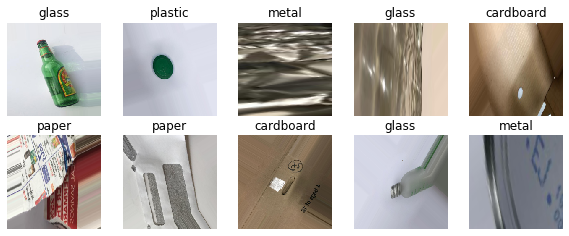
\includegraphics[width=\linewidth]{data/images/03_Dataset/train_sample.png}
    \caption{Sample Training Set from the TrashNet Dataset \cite{yang2016classification}}
    \label{fig:TrainSample}
\end{figure}

\section{ Methods }
In this section, we describe different ways to generate a collage, and methods for classifying and localizing objects in a image. 

\subsection{Single Object in a Images}
This is a baseline, a image has only single object. We take a single image and 

\subsection{Multiple Objects in a Image}
\label{sec:GeneratingCollage}

\subsubsection{Random Collage Generation}
We have a hand labelled masks of foregrounds 



\begin{figure}
    \centering
    \begin{subfigure}{0.3\linewidth}
    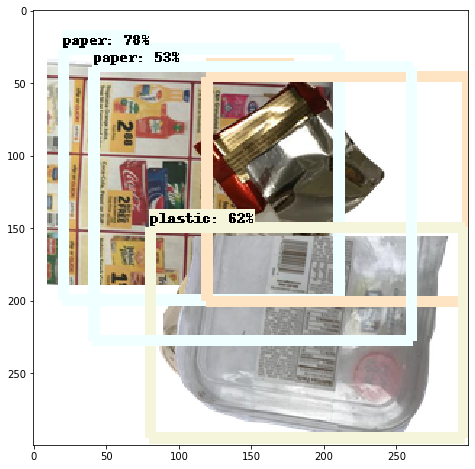
\includegraphics[width=\linewidth]{data/images/04_random_collage/Output_1.png}
    \caption{Detection and Localization Output}
    \end{subfigure}
    \begin{subfigure}{0.3\linewidth}
    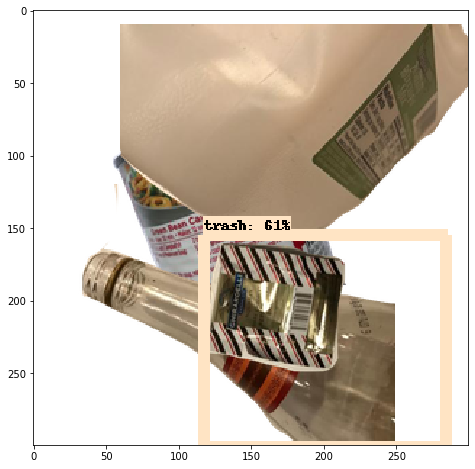
\includegraphics[width=\linewidth]{data/images/04_random_collage/Output_2.png}
    \caption{Detection and Localization Output}
    \end{subfigure}
    
    \label{fig:random_collage}
\end{figure}


%Add figure over here

\subsubsection{Learned Collage}
% Add 2 branch network
Here we try to pose the problem of generating collage as a Knapsack problem. We want to optimize the collage such that the overlap between the two images is minimized. To do this we first get foreground masks of the original image. Since the images in the dataset are not centered, we register all the images such that the bounding box starts at the top left corner. We find out the $t_{x}$ and $t_{y}$  from the top left corner of the bounding box. Later by affine transform, we translate the image such that the top left corner is $(0,0)$. Note we have negated the values of  $t_{x}$ and $t_{y}$  to so that the output moves to the top left.

\begin{equation}
\begin{bmatrix}
x'\\
y'
\end{bmatrix}
= 
\begin{bmatrix}
1 & 0 & -t_{x}\\
0 & 1 & -t_{y}
\end{bmatrix}
\begin{bmatrix}
x\\
y\\
1
\end{bmatrix}
\end{equation}

\begin{figure}[h!]
  \centering
  \begin{subfigure}[b]{0.2\linewidth}
    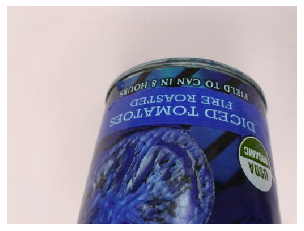
\includegraphics[width=\linewidth]{data/images/04_Learned_Collage/base_original.png}
     \caption{Original Image}
  \end{subfigure}
  \begin{subfigure}[b]{0.2\linewidth}
    
\includegraphics[width=\linewidth]{data/images/04_Learned_Collage/original_mask.png}
    \caption{Registered mask}
  \end{subfigure}
  \begin{subfigure}[b]{0.2\linewidth}
    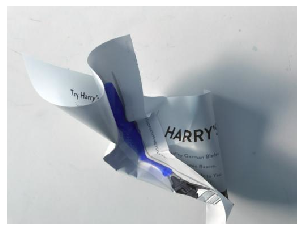
\includegraphics[width=\linewidth]{data/images/04_Learned_Collage/original_target.png}
    \caption{Image to collage}
  \end{subfigure}
  \begin{subfigure}[b]{0.2\linewidth}
    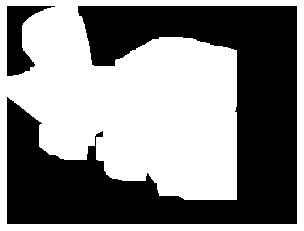
\includegraphics[width=\linewidth]{data/images/04_Learned_Collage/target_mask.png}
    \caption{Registered mask}
  \end{subfigure}
  \caption{Collecting the data to set up the problem}
  \label{fig:learning_collages}
\end{figure}


Now we define a collage loss, so that we have minimum overlap and maximum union area between the foreground. 
\begin{equation}
intersection = base_{mask} \bigcap target_{mask}
\end{equation}

\begin{equation}
union = base_{mask} \bigcup target_{mask}
\end{equation}

\begin{equation}
collage_{loss} = \frac{intersection}{union}
\end{equation}

For every ground truth, we define following anchor points by defining a grid over the image, and then finding the above loss function for each of these points. 

\begin{equation}
anchor_{loss} = 
\begin{bmatrix}
l_{1} l_{2} l_{3} \ldots 
\end{bmatrix}
\end{equation}

\begin{equation}
    optimal_{anchor} = argmin(anchor_{loss})
\end{equation}

We use this optimal anchor point as the ground truth for our learning the optimal place for placing the target. A sample output is shown on page \pageref{fig:learned_collage_output}

\begin{figure}

    \begin{subfigure}{0.2\linewidth}
    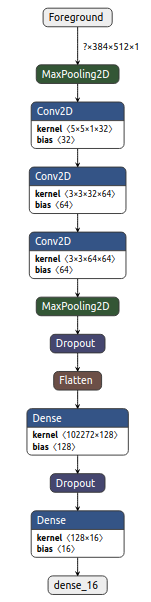
\includegraphics[width=\linewidth]{data/images/04_Learned_Collage/optimization_network.png}
     \caption{Optimization Network}
  \end{subfigure}
  \begin{subfigure}{0.7\linewidth}
    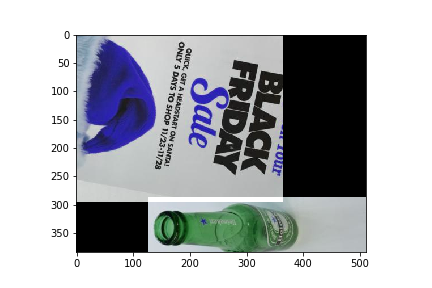
\includegraphics[width=\linewidth]{data/images/04_Learned_Collage/collage_optimization_output.png}
    \caption{Collage of learned network}
  \end{subfigure}
    \label{fig:learned_collage_output}
    \caption{Learned network and sample output collage}
\end{figure}

Though this approach was promising at first, it did not work for the following reasons. 

\begin{itemize}
    \item Since we registered the images, the output location was always the same. All generated collages looked very similar. 
\end{itemize}



% Learning homography transforms using STN

\subsubsection{Blending collages}
To blend different masks on a collage we experimented with a pre-trained GP-GAN \cite{wu2019gp}. A sample output can be seen in \pageref{fig:GAN_Blending}



\begin{figure}
  \centering
  \begin{subfigure}[b]{0.2\linewidth}
    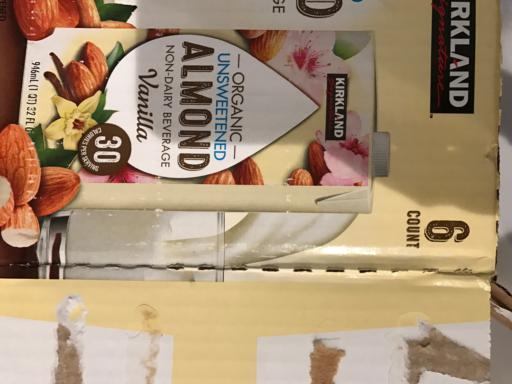
\includegraphics[width=\linewidth]{data/images/04_GP_GAN/cardboard254.jpg}
     \caption{Original Image}
  \end{subfigure}
  \begin{subfigure}[b]{0.2\linewidth}
    
\includegraphics[width=\linewidth]{data/images/04_GP_GAN/mask_display.png}
    \caption{Mask to blend}
  \end{subfigure}
  \begin{subfigure}[b]{0.2\linewidth}
    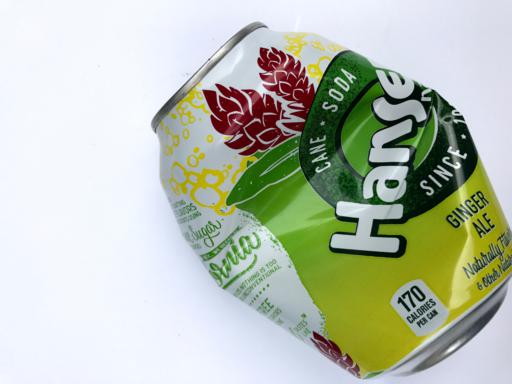
\includegraphics[width=\linewidth]{data/images/04_GP_GAN/metal14.jpg}
    \caption{Target Image to Blend}
  \end{subfigure}
  \begin{subfigure}[b]{0.2\linewidth}
    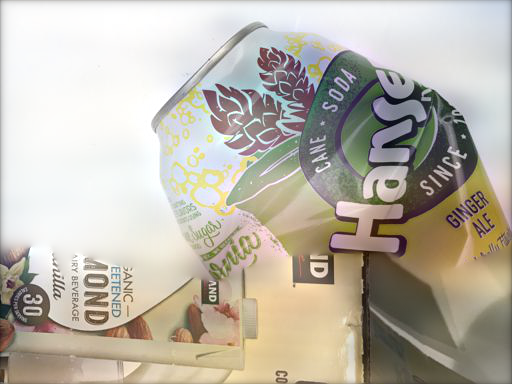
\includegraphics[width=\linewidth]{data/images/04_GP_GAN/result-cardboard331-metal14.png}
    \caption{Result blend}
  \end{subfigure}
  \caption{Collecting the data to set up the problem}
  \label{fig:GAN_Blending}
\end{figure}


\section{Classification of Objects}
TrashNet \cite{yang2016classification} reports only 63\% accuracy for classification on the test set, this can be mainly attributed to its comparatively simple CNN model. We reproduced the results from \cite{CollinChing} where ResNet34 was used to do classification of objects in TrashNet dataset  \cite{yang2016classification} and got better results than \cite{CollinChing}. 

As ResNet \cite{he2016deep} performs better on image classification tasks, we applied transfer learning on ResNet models with weights pre-trained on ImageNet dataset as a baseline. We froze all the layers except the fully connected layers at the top, and the network was finetuned to TrashNet dataset. 

We experimented with different number of layers of ResNet. We noticed that using deeper ResNet does not yield significant improvements in test set accuracy and concluded that ResNet34 was a good sweet spot. 

We used FastAI \cite{howard2018fastai} library to search for an optimum learning rate and fit using one cycle optimization algorithm \cite{1CyclePolicy}. The plots of losses and other metrics are shown below. 

\subsection{Hybrid Transfer Learning}
We use a Hybrid approach to Transfer Learning from \cite{geron2019hands}. For trying this out, we start with pretrained models on image net. Then add a Global Average Pooling layer, followed by Batch Normalization, then Dense output layer. We start by freezing all base layers, and training the output layer by a large learning rate, then after a few epochs, we 

\begin{algorithm}[H]
\SetAlgoLined
\KwResult{Learned Model }
 base =  pretrained model \;
 
 avg = GlobalAveragePooling(base) \\
 reg = BatchNormalization(avg)
 output = Dense(number of classes, activation="softmax", input=reg)

 Freeze base layers of the downloaded model\;

 \While{epochs < 10}{
 train the model with a very high learning rate; 
 }
 
 Unfreeze all base layers; 
 
 \While{epochs < 100}{
 train the model with a very low learning rate; 
 }
 \caption{Hybrid transfer learning}
\end{algorithm}

The advantage of this approach is that it does not change the weights of the base layers drastically in the first few epochs when the last few layers have not yet stabilized. 

\section{Experiments/Results/Discussion}

\subsection{Learning Rates}

\begin{itemize}
    \item LR-Find
    \item LL Decay
    \item Reduce Learning Rate on Plateau
    \item Learning Rate Schedule
    
\end{itemize}

Comparison between different classification algorithms

\begin{figure}
    \centering
    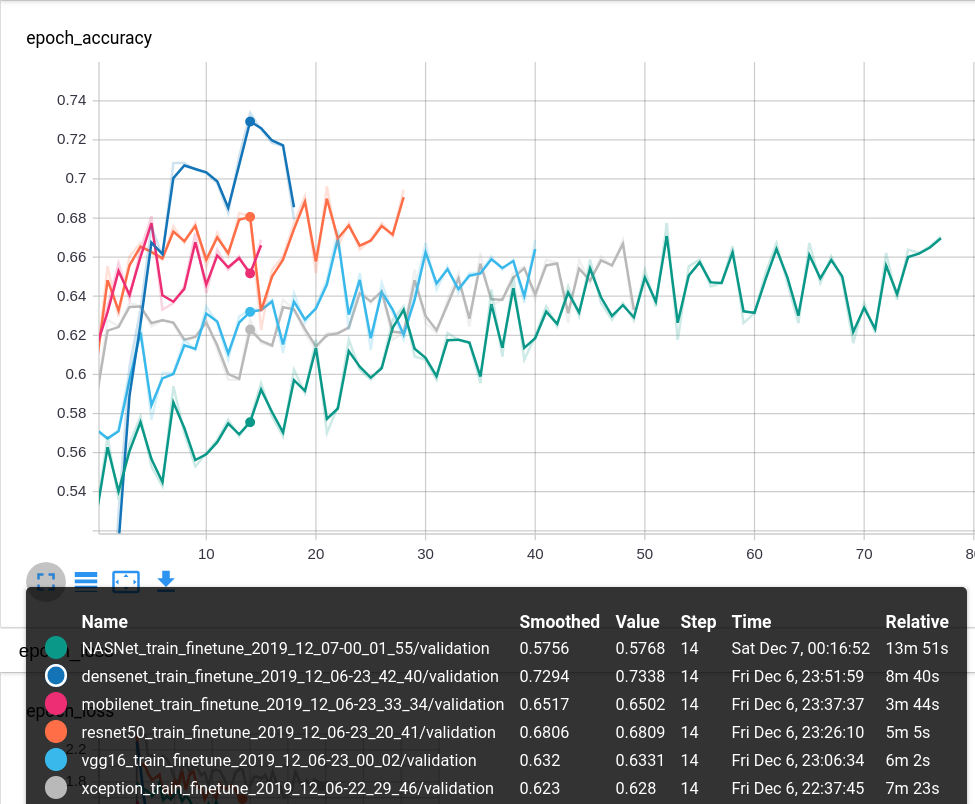
\includegraphics[width=\linewidth]{data/images/05_Comparision/Classification_plot.png}
    \caption{Comparing of validation accuracy between different classification learning algorithms. \cite{Zoph_2018}  \cite{Huang_2017} \cite{howard2017mobilenets} \cite{he2016deep} \cite{simonyan2014deep} \cite{chollet2017xception} }
    \label{fig:my_label}
\end{figure}

We can see that the DenseNet has the highest validation accuracy. We also see different number of epochs, this is because we are using EarlyStopping \cite{geron2019hands}, hence if the validation accuracy does not imporve we stop the training to save time and compute resources. 


\begin{tabular}{lrrrrrrrrr}
\toprule{} &  cardboard &      glass &      metal &      paper &    plastic &  trash &  accuracy &   macro avg &  weighted avg \\
\midrule
precision &   0.130435 &   0.129032 &   0.148936 &   0.196429 &   0.272727 &    0.0 &   0.16092 &    0.146260 &      0.152524 \\
recall    &   0.120000 &   0.160000 &   0.269231 &   0.354839 &   0.081081 &    0.0 &   0.16092 &    0.164192 &      0.160920 \\
f1-score  &   0.125000 &   0.142857 &   0.191781 &   0.252874 &   0.125000 &    0.0 &   0.16092 &    0.139585 &      0.138775 \\
support   &  25.000000 &  25.000000 &  26.000000 &  31.000000 &  37.000000 &   30.0 &   0.16092 &  174.000000 &    174.000000 \\
\bottomrule
\end{tabular}

%From format ------- TO BE REMOVED
You should also give details about what (hyper)parameters you chose (e.g. why did you
use X learning rate for gradient descent, what was your mini-batch size and why) and how
you chose them. What your primary metrics are: accuracy, precision,
AUC, etc. Provide equations for the metrics if necessary. For results, you want to have a
mixture of tables and plots. If you are solving a classification problem, you should include a
confusion matrix or AUC/AUPRC curves. Include performance metrics such as precision,
recall, and accuracy. For regression problems, state the average error. You should have
both quantitative and qualitative results. To reiterate, you must have both quantitative
and qualitative results! If it applies: include visualizations of results, heatmaps,
examples of where your algorithm failed and a discussion of why certain algorithms failed
or succeeded. In addition, explain whether you think you have overfit to your training set
and what, if anything, you did to mitigate that. Make sure to discuss the figures/tables in
your main text throughout this section. Your plots should include legends, axis labels, and
have font sizes that are legible when printed.
%------- TO BE REMOVED



\section{Conclusion/Future Work }
%From format ------- TO BE REMOVED
Summarize your report and reiterate key points. Which algorithms were the highestperforming?
Why do you think that some algorithms worked better than others? For
future work, if you had more time, more team members, or more computational resources,
what would you explore?
%------- TO BE REMOVED



\section{Contributions}
%From format ------- TO BE REMOVED
The contributions section is not included in the 5 page limit. This section should describe
what each team member worked on and contributed to the project.
%------- TO BE REMOVED



\section*{References}

%From format ------- TO BE REMOVED
This section should include citations for: (1) Any papers mentioned in the related work
section. (2) Papers describing algorithms that you used which were not covered in class.
(3) Code or libraries you downloaded and used. This includes libraries such as scikit-learn, Tensorflow, Pytorch, Keras etc. Acceptable formats include: MLA, APA, IEEE. If you
do not use one of these formats, each reference entry must include the following (preferably
in this order): author(s), title, conference/journal, publisher, year. If you are using TeX,
you can use any bibliography format which includes the items mentioned above. We are excluding
the references section from the page limit to encourage students to perform a thorough
literature review/related work section without being space-penalized if they include more
references. Any choice of citation style is acceptable
as long as you are consistent. 
%------- TO BE REMOVED

\medskip


\bibliographystyle{apalike} %other styles produce (author?)
\bibliography{references}

\end{document}